\documentclass[UTF8,11pt,a4paper]{ctexart}
\usepackage[a4paper,margin=20mm,headheight=15pt]{geometry}
\usepackage{graphicx}
\usepackage{subcaption}
\usepackage{booktabs}
\usepackage{array}
\usepackage{xcolor}
\usepackage{hyperref}
\usepackage{fancyhdr}
\usepackage{enumitem}
\usepackage{microtype}
\graphicspath{{figures/project_summary/}}
\hypersetup{colorlinks=true,linkcolor=blue!55!black,urlcolor=blue!55!black}
\setlength{\parskip}{0.45em}
\setlength{\parindent}{1.5em}
\setlist[itemize]{leftmargin=2em,itemsep=0.15em,topsep=0.2em}
\pagestyle{fancy}
\fancyhf{}
\lhead{Drake 语义运动规划项目}
\rhead{阶段工作总结}
\cfoot{\thepage}
\renewcommand{\headrulewidth}{0.4pt}
\newcommand{\metric}[2]{\textbf{#1}：#2}

\title{\vspace{-1.3cm}\Huge 语义约束、C-space 与 GCS\\[0.4em]
\Large Drake 三维移动操作项目阶段总结}
\author{项目工作总览}
\date{2026 年 10 月 11 日}

\begin{document}
\maketitle
\thispagestyle{empty}
\vspace{-0.8cm}
\begin{center}
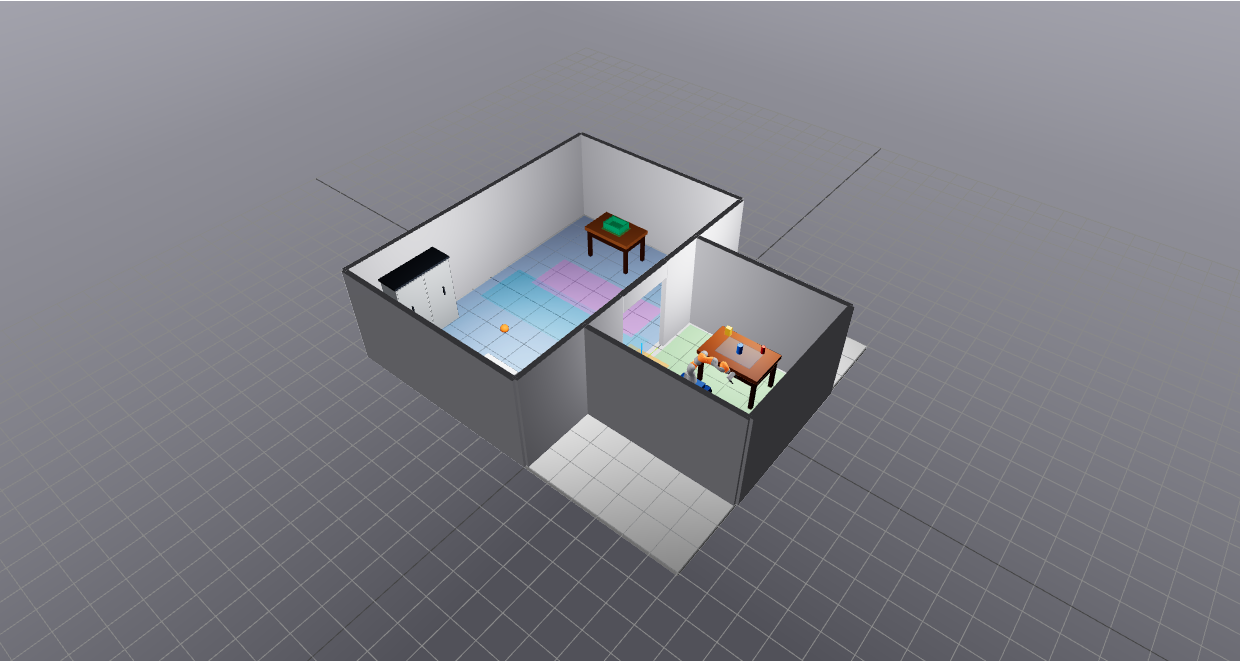
\includegraphics[width=0.94\linewidth,height=0.48\textheight,keepaspectratio]{legacy_two_room_task.png}
\end{center}
\vspace{-0.2cm}
\begin{quote}\small
本项目研究如何把任务语义落到配置空间区域和连续运动轨迹中，并通过 Drake GCS、IRIS-NP2、碰撞审核与接触仿真验证结果。本文汇总主要阶段和证据；不同实验协议的成功率不直接横向合并。
\end{quote}
\begin{center}\small
原始双房间完整取放场景：底盘进入 Room 2 取杯，再把杯子运回 Room 1 放入箱中。\par
\end{center}
\clearpage

\section{项目问题与场景演进}

项目的核心问题分为三层：任务语义是否定义正确；语义允许的 C-space 是否存在连续可行轨迹；GCS 是否相对强基线带来可测量收益。三者不能互相替代。GCS 返回解不自动说明语义建模正确；语义轨迹有效也不单独证明 GCS 比其他方法更好。

\subsection{原始完整任务：底盘进入取物房间}

早期任务为“Room 1 出发 $\rightarrow$ 底盘穿过门洞进入 Room 2 $\rightarrow$ 到桌边 $\rightarrow$ 手臂抓杯 $\rightarrow$ 携杯回 Room 1 并放入箱”。任务谓词包括 \texttt{base\_in\_room1}、\texttt{base\_in\_room2}、\texttt{near\_pickup\_table}、\texttt{cup\_grasped} 和 \texttt{cup\_in\_dropoff\_bin}。

当时房间语义按底盘参考点判断，碰撞检查另行约束机器人几何；并没有严格表达“整台机器人完全处于房间内”，也没有明确要求操作期间整机始终位于某房间。导航 GCS 与后续操作/携物规划主要分阶段执行。这个旧流程已有从初始状态驶入取物区域的连接轨迹，在结构上接近 motion bridge，但当时没有把 bridge 作为独立研究问题提出。

\subsection{后续门口任务：底盘在外、手臂伸入}

根据门口取物讨论，后来另建了一个更强调全臂语义的场景：底盘始终留在 Room 1，手臂从门口进入 Room 2 抓取杯子，再携杯撤回 Room 1。这个任务与原始“底盘进入 Room 2”不同，也与教授最近提出的 green-room toy example 不同。

\begin{figure}[htbp]
\centering
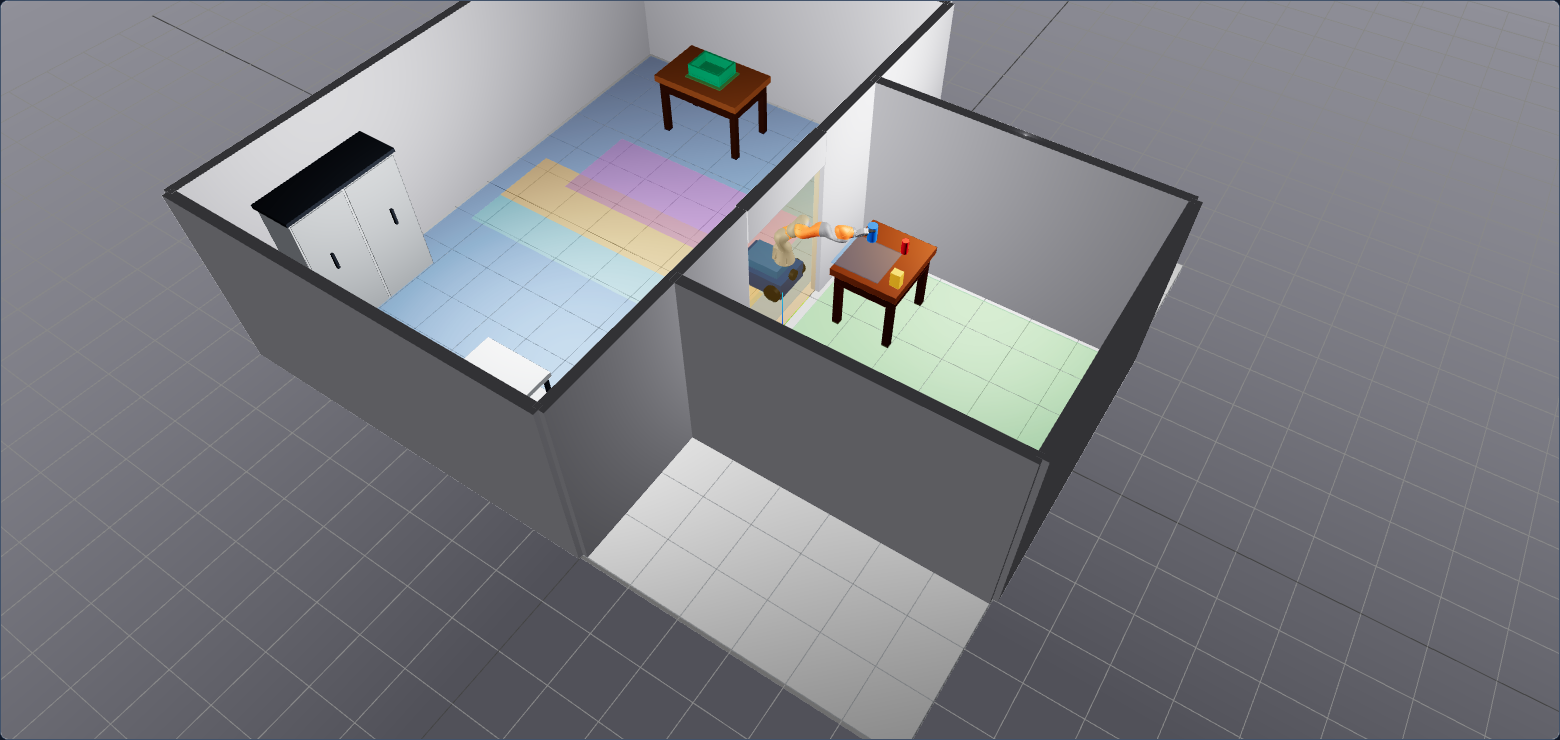
\includegraphics[width=0.96\linewidth]{doorway_reach_gcs_bridging.png}
\caption{当前门口任务的 3D 静帧：底盘停在门外，机械臂跨过门口接近 Room 2 的杯子。该图对应 2026-10-10 的 GCS-Bridging 完整任务结果。}
\end{figure}

\section{已完成的系统工作}

\begin{itemize}
  \item \textbf{Drake 3D 场景：} 两房间、门洞、移动底盘、7-DOF KUKA iiwa、Schunk WSG 夹爪、桌子、杯子、放置箱及环境障碍物；通过 Meshcat 查看和回放。
  \item \textbf{语义建模：} 房间/区域谓词、near-pickup、抓取与携物模式、任务状态机/Product 图、残差和逐帧语义 trace；建立抓取/释放 guard 与独立审核。
  \item \textbf{C-space 与凸区域：} 对底盘导航、机械臂关节空间和携物状态研究凸区域覆盖；采用 Drake IRIS-NP2 生成模式相关区域，以 GCS 选择区域序列并优化连续轨迹。
  \item \textbf{抓取可信度：} 修复过度过滤杯子与夹爪碰撞几何的问题；使用自由杯子接触仿真检查双指接触、抬升、携带与放置，设置张开夹爪负对照。
  \item \textbf{导航覆盖诊断：} 将部分底盘导航从固定朝向 XY 切片扩展到 SE(2) 表达，检查收臂姿态、门洞与障碍物影响。
  \item \textbf{基线与评估：} 构造不调用 GCS 的 Portal/Dijkstra + SOCP 对照；冻结任务集、报告全部失败类别，避免把端点/动作候选失败误报成求解器失败。
\end{itemize}

\section{语义进入 C-space：全臂约束案例}

全臂约束研究固定底盘，分析关节配置是否满足房间边界语义。二维关节切片用于可视化高维 C-space 的局部结构；七关节实验则在关节空间中用 IRIS-NP2 生成区域，并由 GCS 求解轨迹。二维图只是切片，不能代表完整七维 C-space。

\begin{figure}[htbp]
\centering
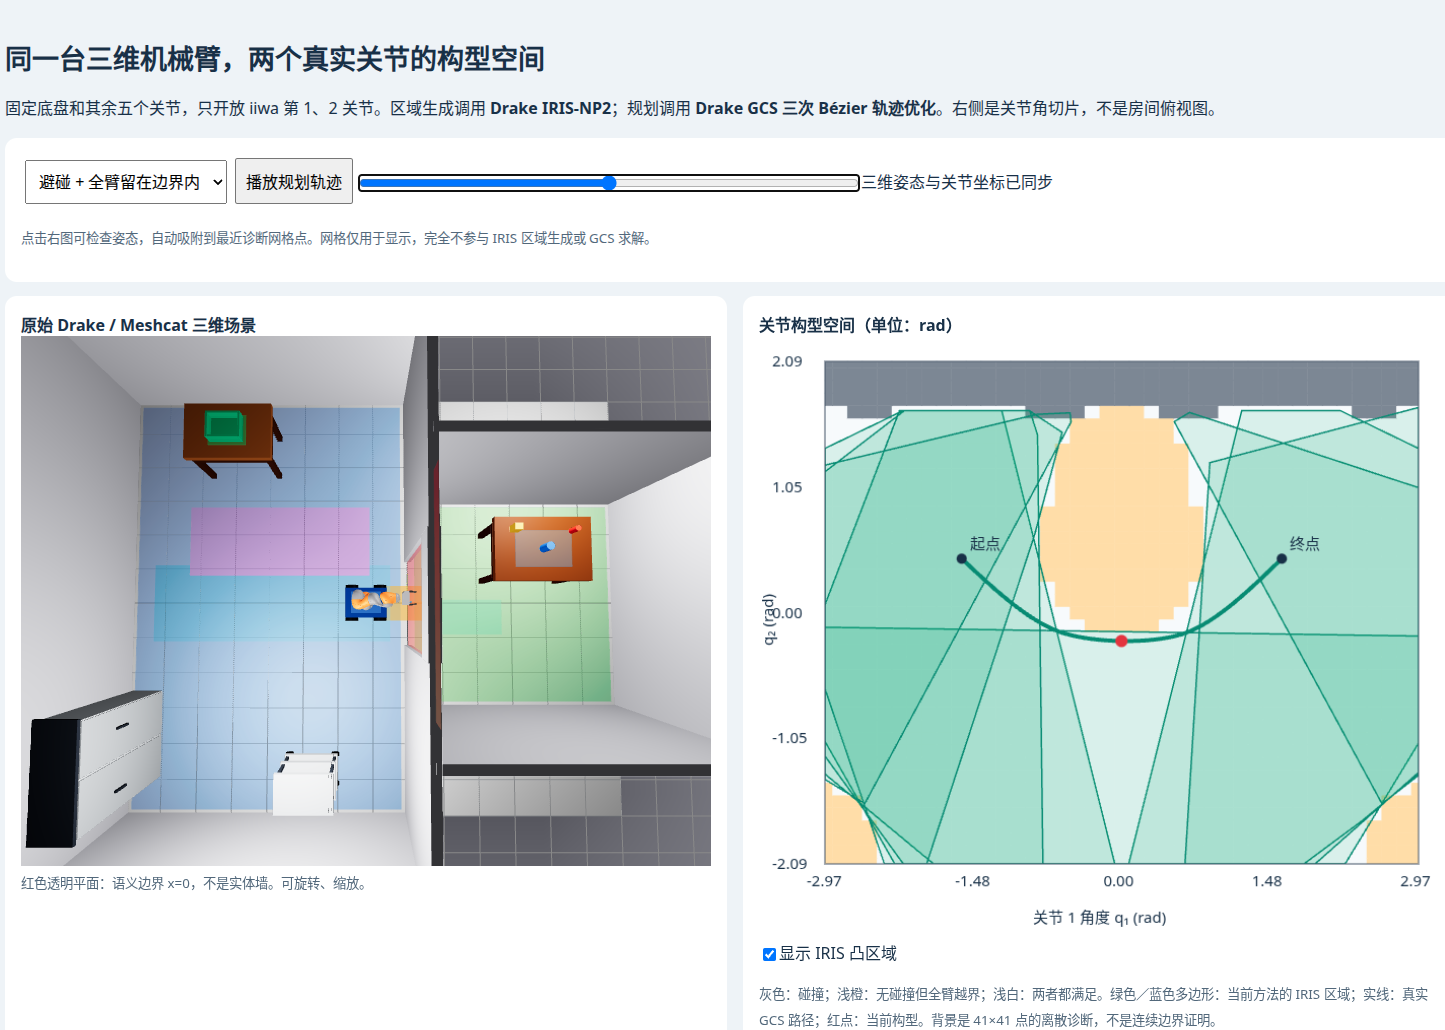
\includegraphics[width=0.98\linewidth]{two_joint_cspace_and_scene.png}
\caption{双关节切片示例：左侧为原始三维场景，右侧为两个真实关节构成的二维切片及凸区域/规划路径。区域背景以有限网格和采样辅助展示，不是连续安全证书。}
\end{figure}

\begin{figure}[htbp]
\centering
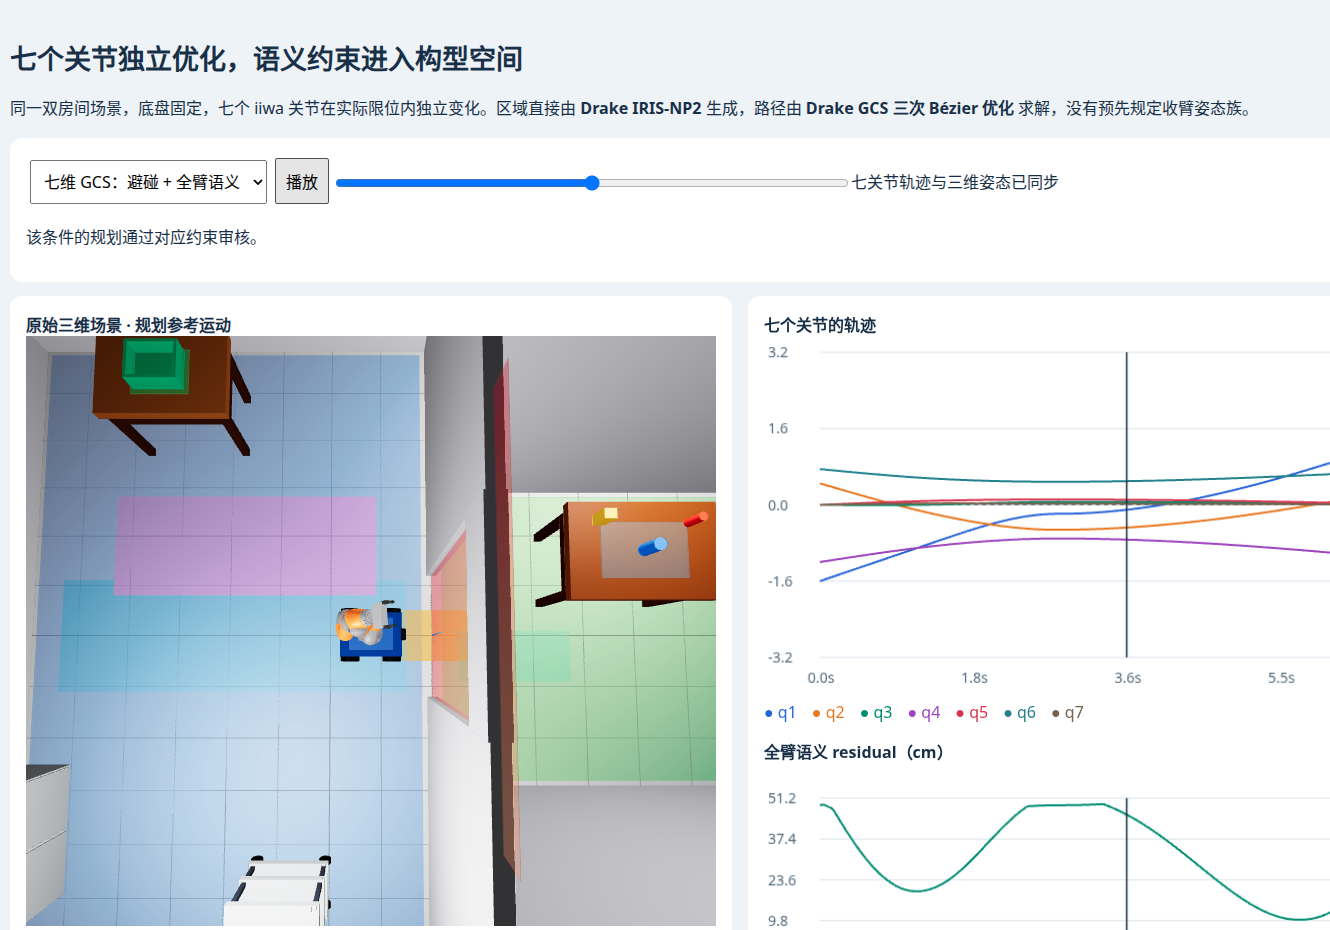
\includegraphics[width=0.98\linewidth]{seven_joint_cspace_and_residual.png}
\caption{七关节全臂语义规划示例：同时展示三维场景、关节轨迹与语义残差。此实验是固定底盘下的 7D 操作空间规划，不是完整 10D 移动底盘动力学规划。}
\end{figure}

\begin{figure}[htbp]
\centering
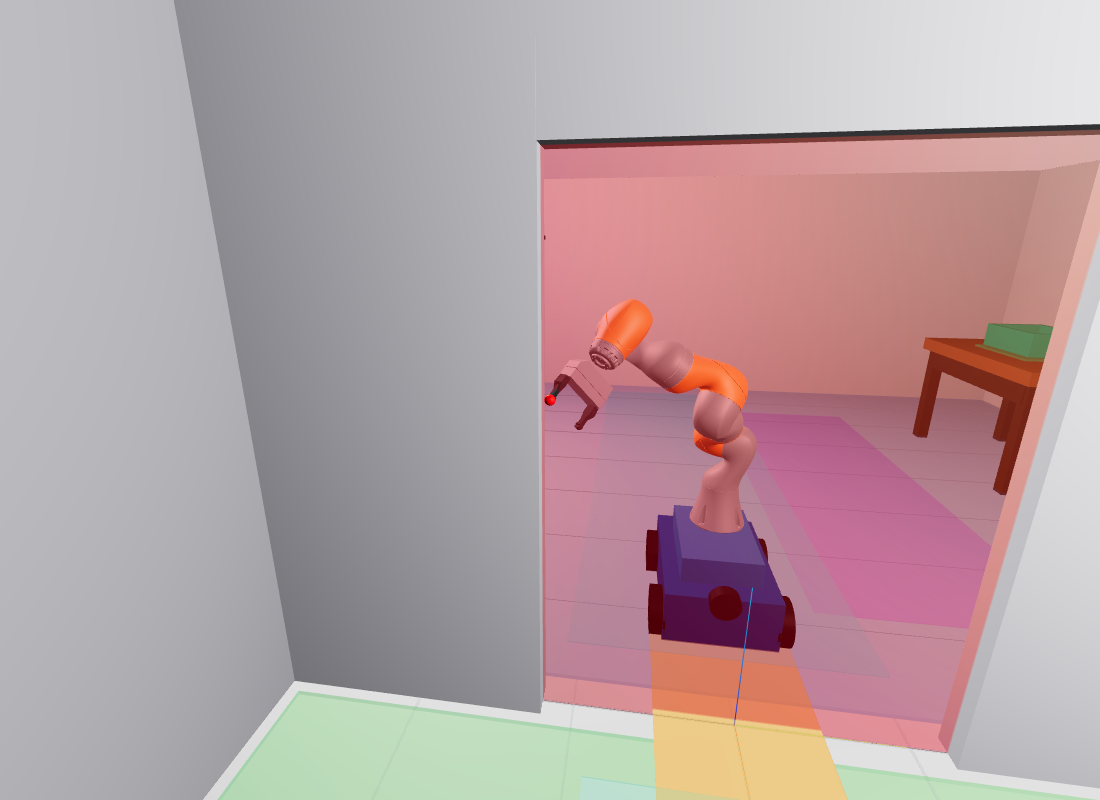
\includegraphics[width=0.58\linewidth]{arm_semantic_boundary_example.png}
\caption{底盘位置不能代表全臂语义：底盘满足房间一侧条件时，机械臂仍可能越过语义边界。}
\end{figure}

\section{接触抓取与执行验证}

规划区域中的“抓取状态”不能代替真实接触证据。项目使用自由杯子与力驱动夹爪进行 SAP 执行，检查双侧指尖接触和携带期间杯子相对夹爪的滑移。局部抓取实验验证杯子可被夹起；完整任务实验则进一步检查携带、放置和释放。

\begin{figure}[htbp]
\centering
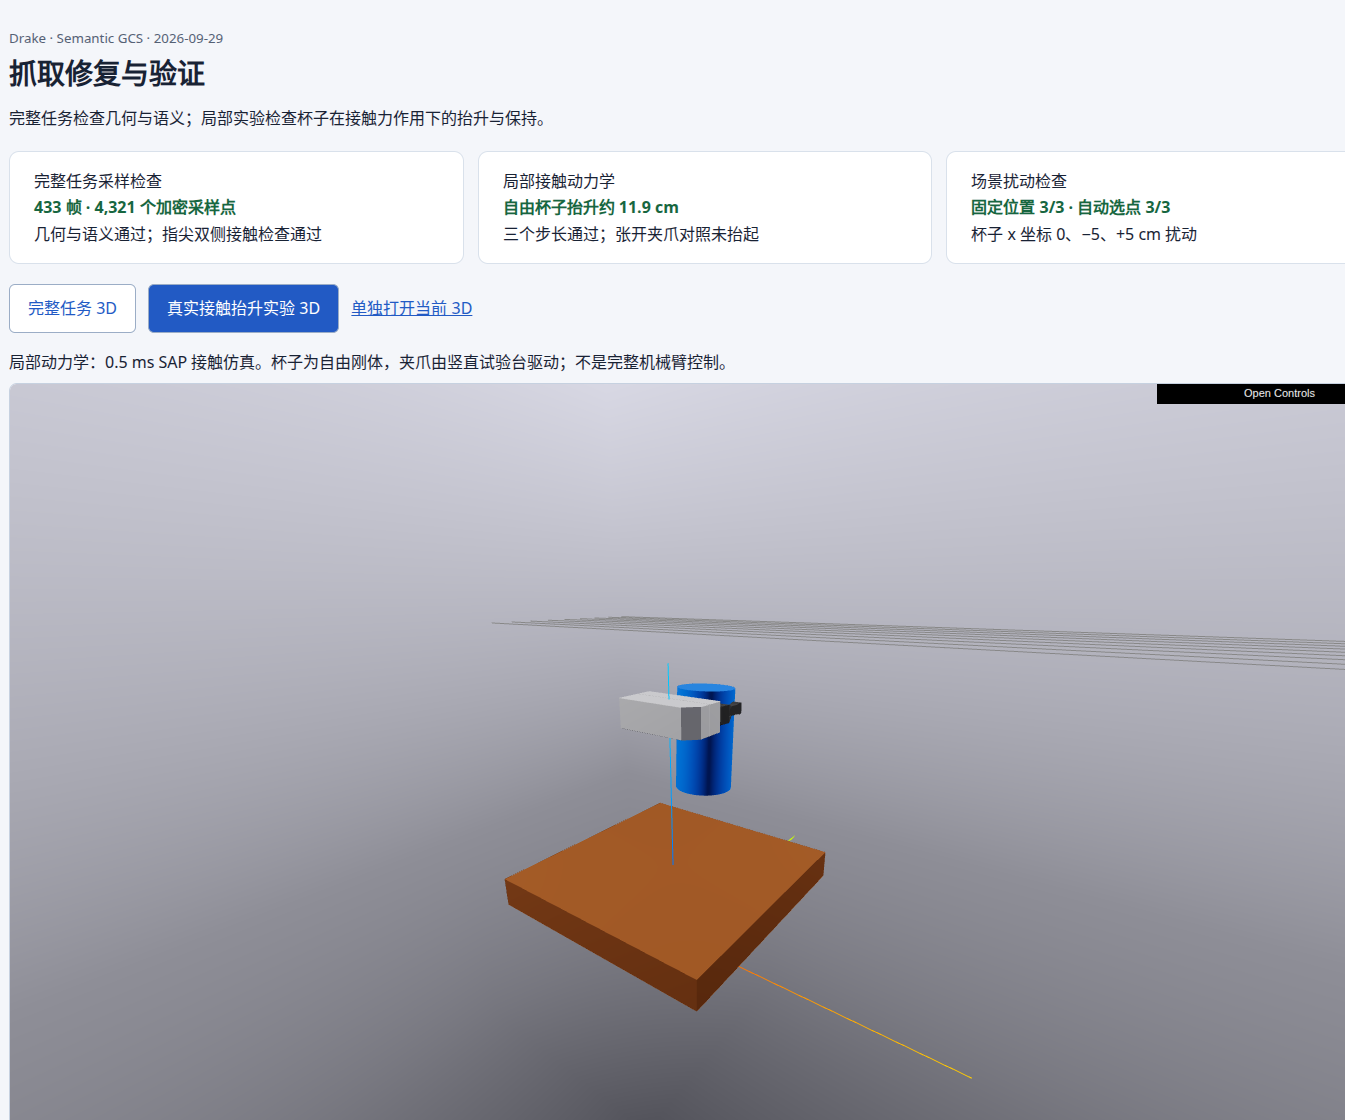
\includegraphics[width=0.91\linewidth]{contact_grasp_validation.png}
\caption{抓取接触修复与验证页面静帧：显示自由杯子、闭合夹爪、局部抬升实验及张开夹爪负对照。局部实验并不等于完整机器人硬件验证。}
\end{figure}

模型边界需要明确：移动底盘是理想全驱动平面模型，不含轮子接触动力学；夹爪/机械臂受到驱动和控制约束，但不等于硬件验证。历史完整任务的部分规划阶段仍使用运动学附着杯模型，独立自由杯接触执行提供的是有限物理执行证据。

\section{语义约束与 GCS 的基线结果}

语义消融实验显示，忽略任务检查点可能得到几何可行、但任务顺序错误的轨迹。另一方面，在现有固定动作和区域库的若干基准中，Product-GCS 与强非 GCS Dijkstra + SOCP 都能完成任务，非 GCS 基线通常更快。因此当前结论是：语义约束对任务有效性有明确作用；现有实验尚未证明 GCS 普遍有更高成功率或更快速度。

\begin{figure}[htbp]
\centering
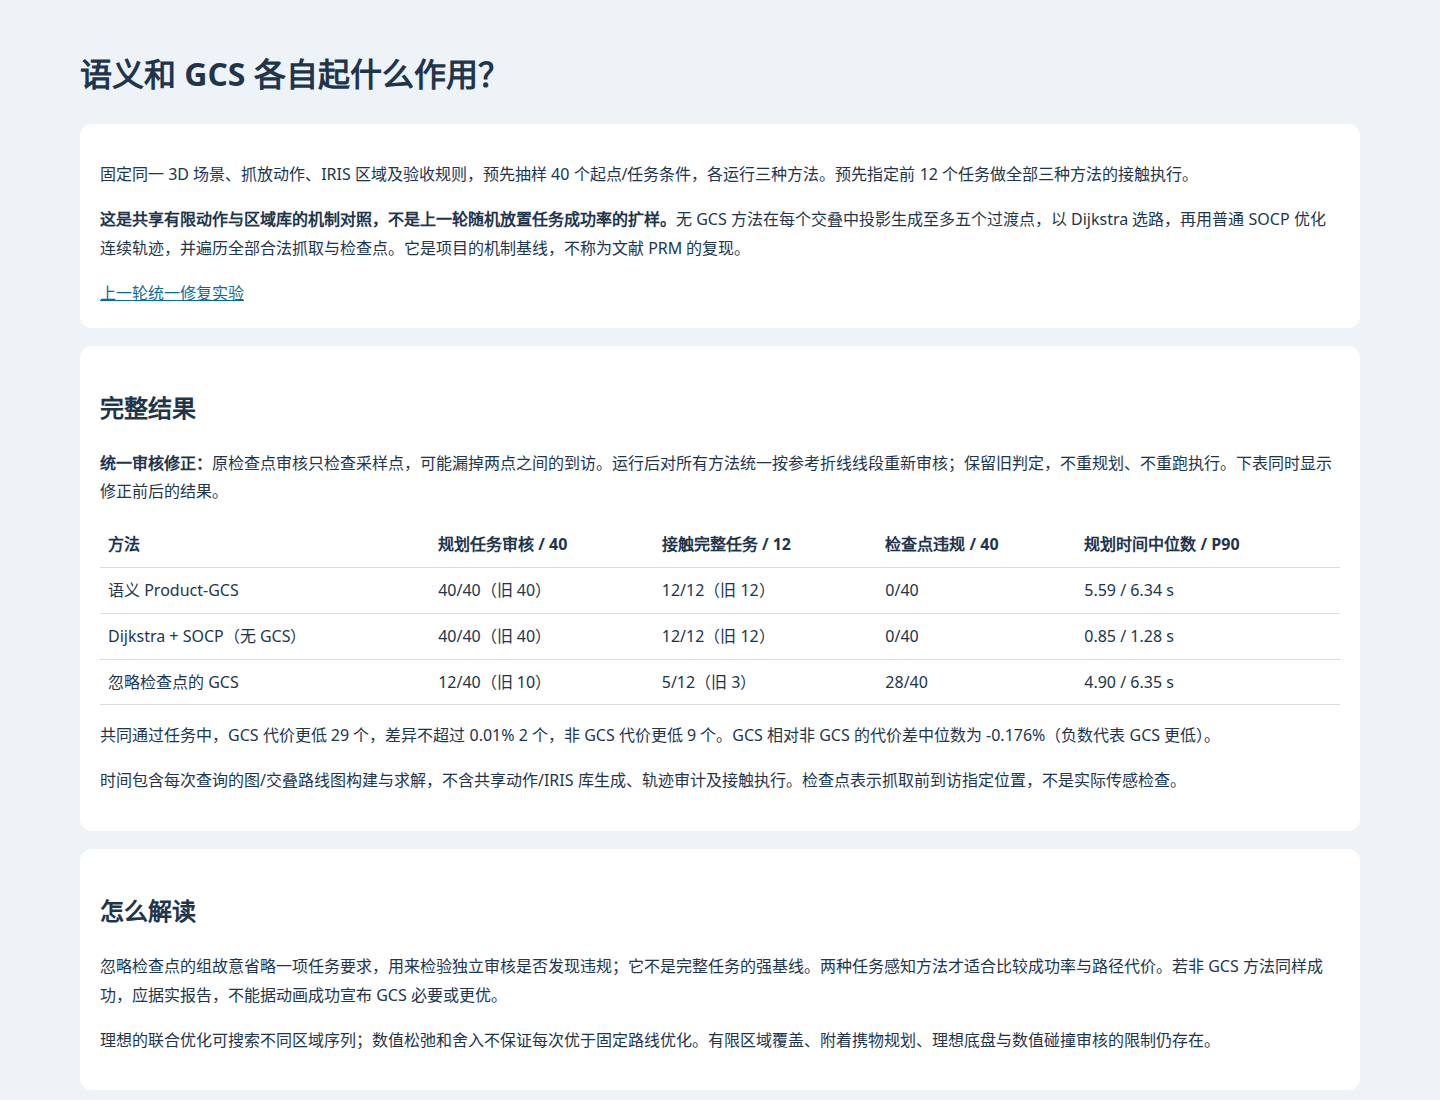
\includegraphics[width=0.85\linewidth]{semantic_gcs_comparison.png}
\caption{同一任务中语义 Product-GCS、Dijkstra + SOCP 与忽略检查点消融的回放/摘要。完整实验统计见报告 47，图中回放截图不能替代完整原始结果。}
\end{figure}

\begin{table}[htbp]
\centering
\small
\begin{tabular}{p{0.27\linewidth}p{0.23\linewidth}p{0.40\linewidth}}
\toprule
实验 & 主要观测 & 结论范围 \\
\midrule
冻结 40 任务评估 & 分阶段 GCS、Product-GCS 各 5/40；在线 IRIS Product-GCS 11/40 & 区域在线修复恢复部分端点覆盖失败；动作候选仍是瓶颈 \\
统一在线修复评估 & 一组 40 个任务上结果从 12/40 到 16/40 & 说明统一动作/区域修复有帮助；不是 GCS 单独优越性的证明 \\
语义机制对照 & 任务感知 GCS 与 Dijkstra + SOCP 均满足语义；忽略检查点的消融出现违规 & 语义会改变任务有效性；GCS 未表现出成功率优势 \\
门口稀疏 reach & 两端点区域起始断连，加入桥接区域后连通并找到轨迹 & 当前场景中凸覆盖可被补连；不等于自动发现所有缺失语义或证明区域全域安全 \\
\bottomrule
\end{tabular}
\caption{代表性历史结果。各行来自不同实验协议，不可把成功率直接相加或作为同一基准排序。}
\end{table}

\section{稀疏语义与 Motion Bridge 实验}

教授最近指出，稀疏语义计划未必存在连续 C-space 细化：起点和目标语义区域可能在凸区域图中断开。项目先对 reach 阶段测试不同 C-space guide 密度；2 点和 9 点配置出现区域图断连，5 点和 17 点配置连通。这个结果反映当前凸覆盖生成/连接流程不单调，并不证明真实自由 C-space 断开。

随后按 GCS-Bridging 论文的连接修复思路，从两个分离 IRIS-NP2 分量中选择最近见证点，检查 DirectLine，并沿通过的路径二分扩张中间 IRIS 区域。初始图有 2 个分量；3 个新增区域后连通，GCS 采用的最短链包含 4 个区域。此例 DirectLine 成功，因此 LocalRRTC 没有运行。

\begin{figure}[htbp]
\centering
\begin{subfigure}[t]{0.32\linewidth}
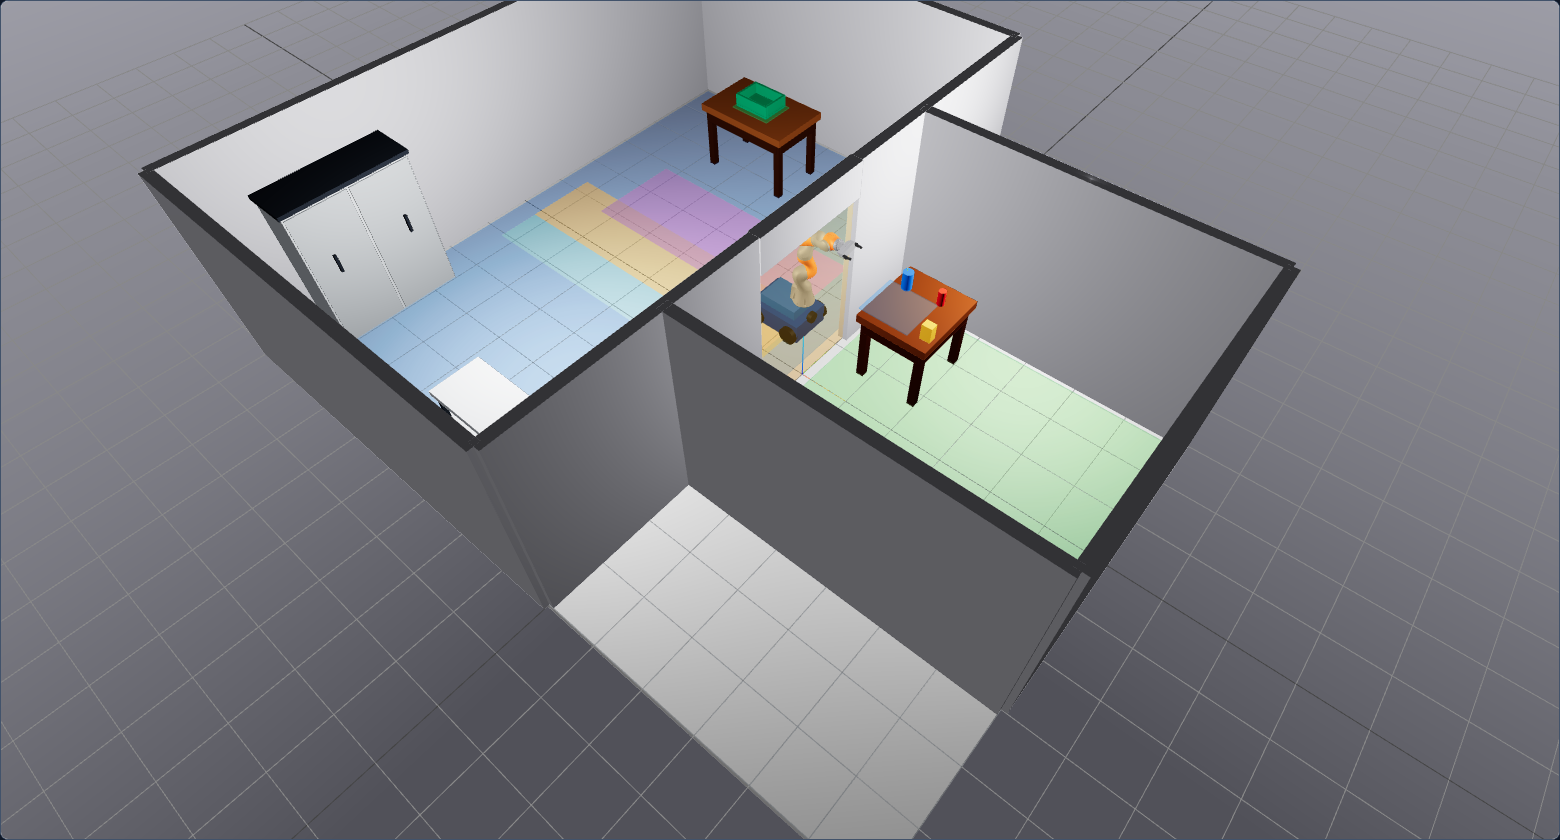
\includegraphics[width=\linewidth]{doorway_phase_reach.png}
\caption{手臂接近杯子}
\end{subfigure}\hfill
\begin{subfigure}[t]{0.32\linewidth}
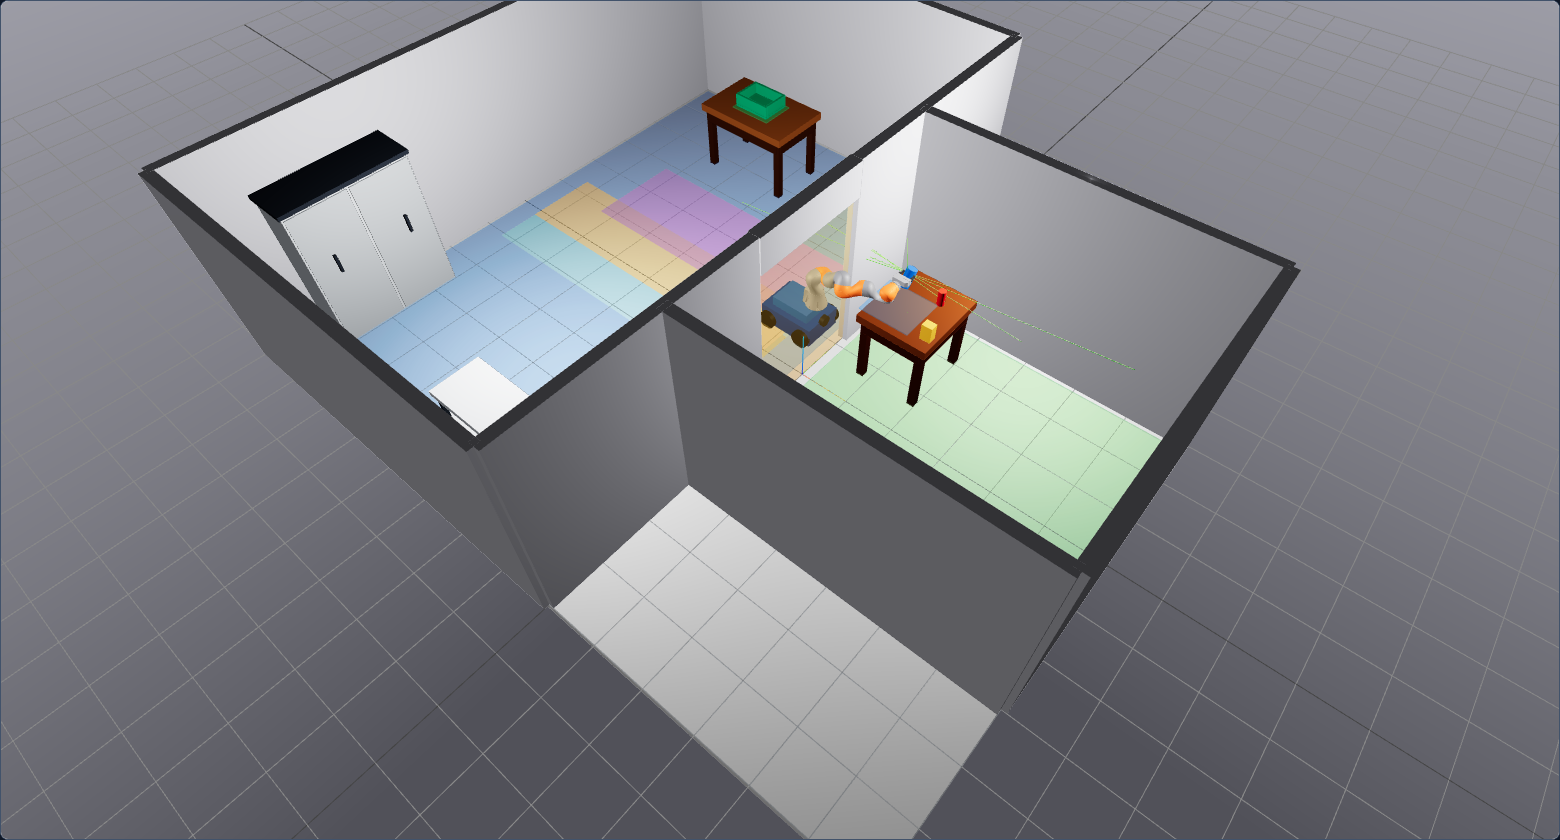
\includegraphics[width=\linewidth]{doorway_phase_grasp.png}
\caption{双指抓取阶段}
\end{subfigure}\hfill
\begin{subfigure}[t]{0.32\linewidth}
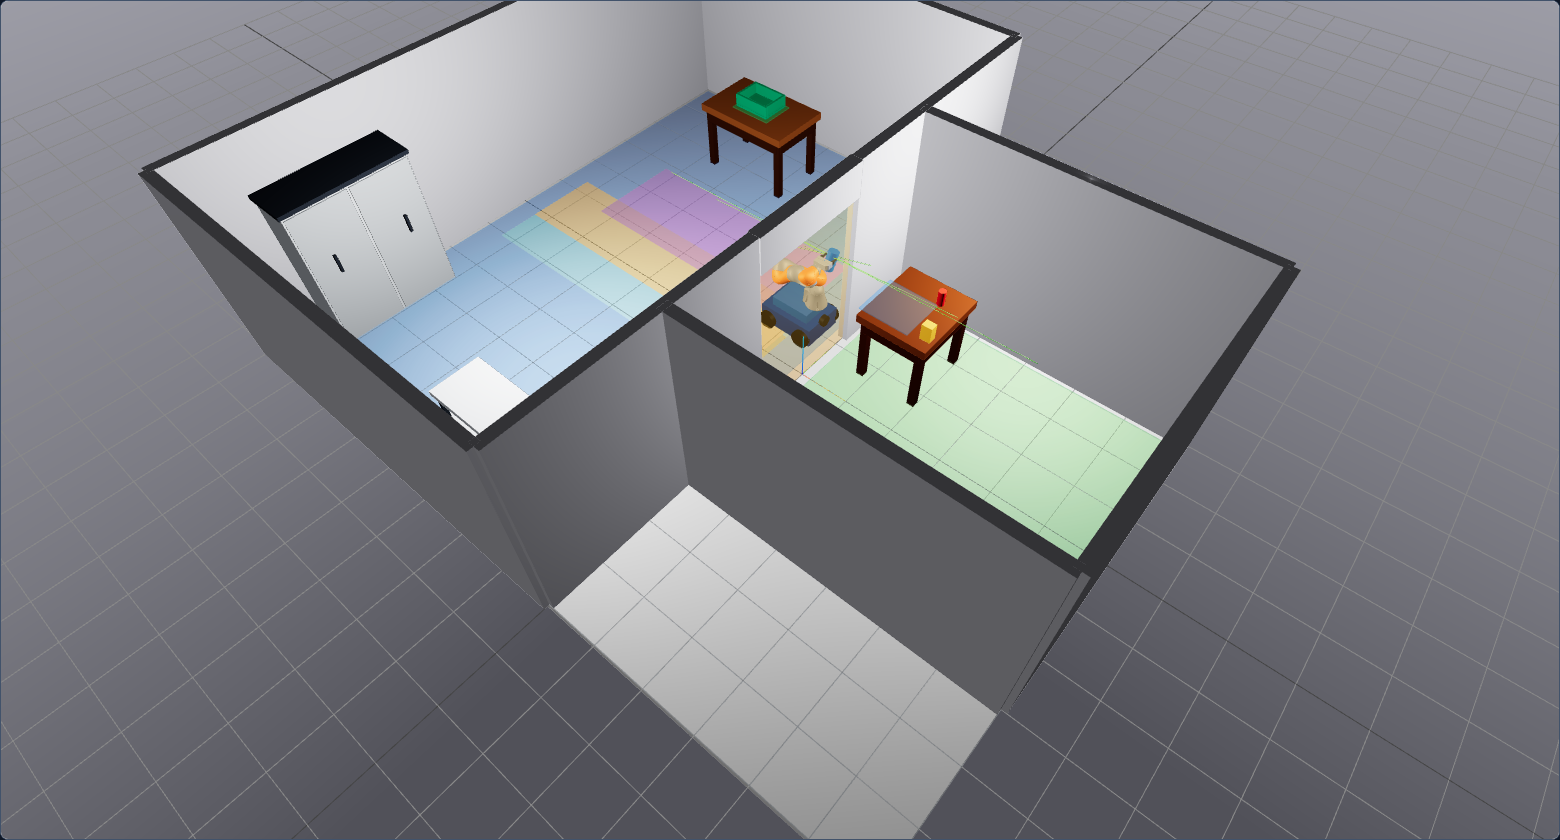
\includegraphics[width=\linewidth]{doorway_phase_retraction.png}
\caption{携杯撤回阶段}
\end{subfigure}
\caption{同一门口场景完整动画的三个时间帧。它们对应“底盘留在 Room 1、手臂进入 Room 2”的任务定义，不是 green-room 全机器人入室任务。}
\end{figure}

在集成版本中，区域生成完成后只调用一次 9D Drake GCS 求解，统一选择 Room 1 底盘移动、自由杯 reach、双指抓取动作和携杯撤回层。SAP 执行审计结果如下：

\begin{itemize}
  \item 底盘到门平面的最小几何间隙：0.146 m；末端进入 Room 2 的最大深度：0.499 m。
  \item 双指真实接触抓住自由杯子，携杯回到 Room 1；执行记录中非预期接触为 0。
  \item 最终轨迹的 142 个保存构型均通过对应碰撞检查；全局 GCS 求解时间约 0.079 s，区域生成时间约 17.31 s。
  \item attached-cup IRIS 区域的 1,600 个独立留出样本中有 3 个碰撞构型。因此只能说所选轨迹的离散检查与 SAP 执行通过，不能把整个区域宣称为严格安全证书。
\end{itemize}

\section{教授最新 green-room toy example：与当前工作区分}

教授当前建议的最小语义结构是：
\begin{enumerate}[leftmargin=2em]
  \item \texttt{whole-robot-inside(green room)}：在机械臂操作开始前，整台机器人进入绿房间；
  \item \texttt{whole-motion-inside(green room)}：机械臂操作期间，整台机器人始终处于房间内。
\end{enumerate}

初始配置在语义有效 C-space 区域之外，所以还需一条从初始配置进入有效区域的 motion bridge。旧版本“底盘进入 Room 2 后停下，再由手臂抓取”的流程与这个结构相近，但旧语义只检查底盘参考点，没有严格落实整机全程在房间内。当前的“底盘在 Room 1、手臂伸入 Room 2”又是另一套语义。后续应按教授最新定义重新明确绿房间、全机器人谓词、运动不变量、桥接条件，再决定是否复用旧场景几何。

\section{主要限制与下一步}

\begin{itemize}
  \item 自然语言指令到谓词和语义任务图仍主要由人工转换。
  \item 局部 C-space 区域图无路径不等于真实任务物理不可行；IRIS 留出抽样也不是区域全域安全证明。
  \item 高密度/离散碰撞检查不是严格连续时间安全证明；SAP 底盘模型不是轮式机器人模型。
  \item 已有 GCS 对照没有证明 GCS 的成功率优势。后续应设计能区分联合区域/连续变量规划与强非 GCS 基线的任务，并固定同一语义、区域库和计算预算。
  \item 优先按 green-room 定义设计新 toy scenario，建立“未加桥接时图不连通 / 加入 motion bridge 后可连续细化”的公平消融，并验证从 bridge 到操作轨迹的连续连接。
\end{itemize}

\clearpage
\section{详细报告与可复查产物}

本 PDF 的截图素材及其来源保存在 \texttt{reports/figures/project\_summary/}。各阶段详细协议、代码和原始记录见后面的报告索引。

关键结果目录：
\begin{quote}\small\ttfamily
outputs/results/\\
doorway\_arm\_reach\_semantic\_v13/gcs\_bridged/
\end{quote}
目录内包含 \texttt{result.json}、\texttt{semantic\_trace.json}、SAP 执行 trace 与 Meshcat HTML 动画。历史结果应结合各自输出目录中的协议、配置快照和源码快照复核。

\subsection*{教授建议的 motion bridge 结构（下一阶段待实现）}
\begin{center}
\fbox{\parbox{0.18\linewidth}{\centering 初始配置\\$q_0$\\在语义区域外}}
\quad$\longrightarrow$\quad
\fbox{\parbox{0.22\linewidth}{\centering 碰撞自由\\motion bridge\\连接到有效区域}}
\quad$\longrightarrow$\quad
\fbox{\parbox{0.21\linewidth}{\centering $S_{\rm green}$\\whole robot inside}}
\quad$\longrightarrow$\quad
\fbox{\parbox{0.23\linewidth}{\centering GCS 操作轨迹\\$q(t)\in S_{\rm green}$}}
\end{center}
\small
该图概括教授提出的 toy task，而不是当前已完成的门口伸手场景。bridge 负责从初始配置连到语义有效区域；进入操作模式后，再要求整台机器人沿 reach/grasp 轨迹持续满足房间语义。
\normalsize

\subsection*{报告与论文入口}
\begin{itemize}
  \item 抓取与接触：报告 05--07；全臂语义和 C-space：报告 30--36。
  \item 任务评估与 GCS 基线：报告 44、46--51；项目交接：报告 52、56。
  \item 稀疏连通性和门口演示：报告 58--60；本项目图文总览：报告 61。
  \item 参考论文：\href{https://arxiv.org/abs/2205.04422}{GCS motion planning}；\href{https://arxiv.org/abs/2303.14737}{IRIS-NP}；\href{https://arxiv.org/abs/2608.22326}{GCS-Bridging}。
\end{itemize}

\vfill
\begin{center}\small\color{gray}
总结范围：截至 2026 年 10 月 11 日的项目工作区与报告 01--60。数值结果均按各自协议报告；本文不声称普遍最优性、完备性或连续时间安全保证。
\end{center}

\end{document}
